\documentclass{article}
\usepackage{float} 
\usepackage{subfigure}
\usepackage{graphicx}
\usepackage{CTEX}

\begin{document}

\section{特征预处理}

连续型特征经归一化处理:
$$
\tilde{x} = \frac{x - \mu}{\sigma}
$$
其中,$\mu$为列$x$的平均值,$\sigma$为列$x$标准差。

类型特征未经处理。

训练神经网络模型时,合并红酒和白酒数据集,以求同时获得更多数据。合并后加入类型特征,标注该数据来自红酒还是白酒数据集。

\section{基本方法和算法推导}
\subsection{神经网络模型}

神经网络模型结构如下:

\begin{enumerate}
    \item 输入层:线性层,输入个数为12,输出长度为4
    \item 2个隐藏层:线性层,输入长度为4,输出长度为4
    \item 输出层:Softmax,输出长度为11
\end{enumerate}

其中,线性层的激活函数均为ReLU。模型输出Softmax多类分类结果,计作$\left\{\hat y_i\right\}_{i=0}^{i=11}$,$\hat y_i$表示预测品质分数为$i$的概率。取概率最大对应的$i$为模型预测输出,即$prediction=\arg_i\max \hat y_i$。计算损失函数时,将品质分数真实值转化为onehot编码向量,从而和模型输出具有相同含义。损失函数取交叉熵损失:
$$
L = \sum_i y_i \log(\hat y_i)
$$
由于$y_i$事实上为onehot编码,只有一项$y_i=1$。

训练采用mini batch的随机梯度下降算法,取batch大小为256,最大迭代次数为1000,学习率为$4\times10^{-4}$。

\section{结果分析}
\subsection{神经网络模型}

训练前将数据集分隔为训练集和测试集,测试集大小取为原数据集大小的10\%,在测试集计算模型输出准确率,只有模型输出和真实值相同,才认为模型预测准确。得到模型准确率为52\%,效果不佳。画出模型训练过程中,损失函数值变化趋势,如图\ref{fig:loss}。反映出损失函数在一定时间后不再变化。

\begin{figure}[htbp] %H为当前位置,!htb为忽略美学标准,htbp为浮动图形
    \centering %图片居中
    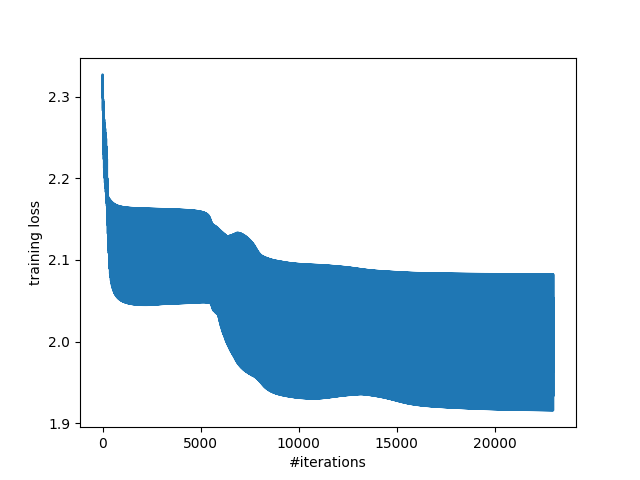
\includegraphics[width=0.4\textwidth]{loss_plot.png}
    \caption{损失函数值变化}
    \label{fig:loss}
\end{figure}

\end{document}
